\documentclass[a4paper, 12pt]{article}
\usepackage[T1]{fontenc}
\usepackage{graphicx}
\usepackage[utf8]{inputenc}
\usepackage{lmodern}

% IF YOU WANT TO USE ENGLISH OR SWEDISH, CHANGE HERE
\usepackage[swedish]{babel}
%\usepackage[english]{babel}


\usepackage{amsmath , amssymb , amsthm}
\usepackage{relsize}
\usepackage{caption}
\usepackage{subcaption}
\usepackage{float}
\usepackage{hyperref}
\usepackage{multirow}
\usepackage{verbatim}
\usepackage{pdfpages}
\usepackage[document]{ragged2e}
\newcommand{\HRule}{\rule{\linewidth}{0.2mm}}
\newcommand{\tabitem}{~~\llap{\textbullet}~~}
\usepackage[margin=0.977in]{geometry}
\usepackage[utf8]{inputenc}
\usepackage{indentfirst}
\usepackage{cases}
\usepackage{breqn}
\usepackage{dirtytalk}
\usepackage{amsmath}
\usepackage{natbib}
\usepackage[nottoc]{tocbibind}
\usepackage{lipsum, babel}
%\bibliographystyle{abbrvnat}
\bibliographystyle{agsm}
\setcitestyle{authoryear,open={(},close={)}}
\usepackage{fancyhdr}
\pagestyle{fancy} 
\usepackage{wrapfig}

\graphicspath{Images/}

%===================================================
%   Ovan är importerade packet av diverse slag, för den som vill veta vad 
%   alla gör/ger är det bara att söka på valfri sökmotor om dessa.
%   (Blir annars mycket text som ingen vill läsa av er kommer läsa)
%===================================================

\begin{document}
\begin{titlepage}

%===================================================
%   Här skriver ni projektnamn, kursnamn, kurskod
\title{\textbf{Project Group} \\ \textbf{Course Name} \\ Course Code} 

%===================================================
%   Här skriver ni era namn
\author{Jennifer Fredberg \& Johanna Persson}    

%===================================================
%   Datum som kommer stå vid titel sidan
%   Om den lämnas \date{} kommer recompile datumet stå.
\date{\today}

\maketitle
\begin{figure}[H]
\centering

\includegraphics[scale=0.5 ]{Images/Chalmers.png}
\end{figure}
\end{titlepage}

\newpage
%===================================================
%   Innehållsförtekning
\tableofcontents
\newpage

%===================================================
%   \section{namn} är ett nytt kapitel men namn namn
\section{Inledning}



\subsection{Bakgrund}

%I detta avsnitt beskrivs bakgrunden till frågeställningen, det vill säga en kort beskrivning av företagets situation och varför företaget vill ha uppdraget utfört. Observera att det inte är bakgrunden till att studenten gör examensarbetet som ska beskrivas

% Johanna test bakgrund: 
Inom fastighetsautomation används system som kan koppla ihop och samla data från de kopplade enheterna. Ett system som används är SCADA Citect, där projekt delas upp i projektmappar med de tillhörande filerna. Dessa filer kan innehålla bilder, larm och variabler. Datan i projekten kan ändras av flera olika instanser som har tillgång till datan och ändras i dagsläget manuellt av olika personer. Vid den nuvarande inmatningen kan man inte säkerställa att datan matas in på ett korrekt sätt och måste granskas för att kontrollera kvaliten. Fel inmtning kan resultera i att monterade sensorer inte kan användas för att de fått tilldelat ett felaktigt variabelnamn. 
\\[5mm]

I nuläget kontrolleras alla inmatade data manuellt och tar mycket arbetstid. För att autmatisera kontrollen av datakvaliten på datan behövs ett script och användargränssnitt för att kontrollera vilka filer som saknas, tidsstämplar som är annorlunda samt skillnader inne i .dbf-filer (typ av excel-format). På så sätt kan man få en överblick kring vad som ändrats i projekten i form utav nya bilder, larm och ändrade larmprioriteter. Det är i dessa filer som behov av automatisk kontroll eller automatiskt kunna plocka fram två filer för att jämföra för att se om rätt syntax har används vid ändring. Kvalitén på SCADA systemets funktion är beroende av kvalitén på ändringarna av filerna.
test grejs

%I SCADA systemet Citect så byggs projekt upp i form av projektmappar där filer för bilder, variabler och larm sparas. Datan till varje projekt kan ändras på flera olika ställen (olika personer), dvs datan i SCADA systemet där man i dagsläget inte kan garantera kvaliteten på%det som ändras/matas in. Exempelvis vilka filer som saknas, tidsstämplar som är annorlunda samt skillnader inne i .dbf-filer (typ av excel-format). På så sätt kan man få en överblick kring
%vad som ändrats i projekten i form utav nya bilder, larm och ändrade larmprioriteter. Det är
%i dessa filer som behov av automatisk kontroll eller automatiskt kunna plocka fram två filer
%för att jämföra för att se om rätt syntax har används vid ändring. Kvalitén på SCADA
%systemets funktion är beroende av kvalitén på ändringarna av filerna.


%Jennifer test bakgrund (Frågesätlnning lös skiten bara) använt å gjort om lite i den texten vi hade: Acobia är ett företag som skapar smarta lösningar på det man bara vill skall fungera, som infrastruktur och fastigheter. Acobia använder sig i dagsläget av SCADA systemet Citect. I de olika projekten skapas projektmappar, där bland annat filer för bilder, variabler och larm sparas. Då datan till varje projekt kan ändras på flera olika ställen (av olika personer), kan man i dagsläget inte garantera kvaliteten på det som ändras/matas in. Vilket ställer till med problem, exempelvis vilka filer som saknas, tidsstämplar som är annorlunda samt skillnader inne i .dbf-filer (typ av excel-format). Det blir då viktigt för företaget att få en bra överblick kring vad som ändrats i projektet i from av nya bilder, larm och ändrade larmprioriteter. Kvalitén på SCADA systemets funktion är beroende av kvalitén på ändringarna av filerna.
 


%Acobia skapar intelligenta lösningar där affärer, organisationer och system integreras till en smart helhet.

\subsection{Syfte}
%Syftet är en kort beskrivning av uppdraget och vilket resultat uppdraget ska leda till.'

Syftet med arbetet är att skapa ett verktyg där man jämför filer vid olika tider för att se skillnaderna. Kontrollen av datan automatiseras så att mindre arbetstid behöver läggas på att kontrollera inmatade och ändrade värden i projektfilerna.



%För att lösa problemet med försämringen av kavliteten på SCADA systemets funktion kommer en jämförelse att behövas göras mellan den nya och gamla filen. Detta kan göras med en automatisk kontroll eller att automatiskt plocka fram de två filerna för att kunnde jämföra dem för att se om rätt syntax har använts. Ett program som automatiskt jämför filer för att kunna upptäcka de skillnader som uppståt vid filändring kommer att utvecklas. 
\subsection{Avgränsningar}
Under avgränsningar talar man om vad man inte ska behandla.


\begin{itemize}
    \item Vet inte
\end{itemize}


\subsection{Mål}
Målet är att kunna med ett UI och logik bakom kunna jämföra två filer och visa skillnaderna mellan dessa. Det ska även visa vilken version av filerna som öppnas för att kunna följa när de felaktiga ändringarna uppkommer.



//Går det att med filerna presentera skillnaderna mellan dom så att det sparar arbetstid.


//Utifrån syftet ska frågeställningen preciseras, exempelvis genom att skriva ner ett antal frågor //som ska besvaras. Ett annat sätt är att skriva ett antal påståenden (hypoteser) som sedan ska //verifieras eller förkastas under arbetets gång.



\begin{itemize}
    \item Hur delar SCADA upp filerna som uppkommer vid projekt och hur är SCADA systemet uppbyggt?
    \item Hur kan man läsa in en fil?
    \item Hur ska man plocka ut och jämföra två filer?
    \item Hur sparar man och producerar en ny fil (eller på annat sätt) för att visa skillnaderna?
    \item Hur fungerar en databas/filserver?
    \item Hur ska man koppla ovan logik för att kontrollera filerna till ett användbart program?
    \item Går det att sammanställa på ett användarvänligt sätt?
    \item 
    \item 
\end{itemize}


\newpage
\section{Metod}

Metodkapitlet beskriver hur man lägger upp arbetet. Vilket bland annat omfattar arbetsgång, design av experiment och användning av olika metoder för datainsamling. I idealfallet ska ett metodkapitel vara så utförligt att vem som helst med vissa baskunskaper inom området ska kunna utföra arbetet på det sätt som beskrivs och nå samma resultat. Att beskriva metoden är viktigt för att uppdragsgivaren ska kunna bedöma om målet går att nå på det föreskrivna sättet. Därför är det också viktigt att förklara i det här kapitlet varför den valda metoden ger ett tillförlitligt resultat.
\\[5mm]

För att kunna klara av detta arbetet behövs en faktainsamling att göras. Även kvalitativ diskussion mellan grupp medlemmarna samt handledare på företget och Chalmers. I faktainsalmigen kommer internet sökning att användas, då det finns bra och gratis information om programmering i olika språk. Informativa videos kommer också ge oss ökad förståelse innan arbetet kan dra igång. Då det finns många open soruces online där man kan ta del av andras kunskap är detta ett bra sätt att lära sig på. 

\\[5mm]
När väl faktainsamlingen är gjord kan man börja med att programmera ett program som kommer jämföra filer.För att automatiserad kontroll kommer kunna vara genomförbar. Under tiden kommer en fortsatt diskussion ske mellan de iblandade, för att kunna få inputs under arbetsgången. Genom att man succesivt testar programmeringen och sparar denna i versions filer under programmeringens gång kommer man kunna få ett bra slutresultat. 


\newpage
\section{Tidplan}


\newpage
%\section{Math}
There are a few tricks to fixing the figures in your report, here we will show some of them.

\begin{figure}[H]
    \centering
    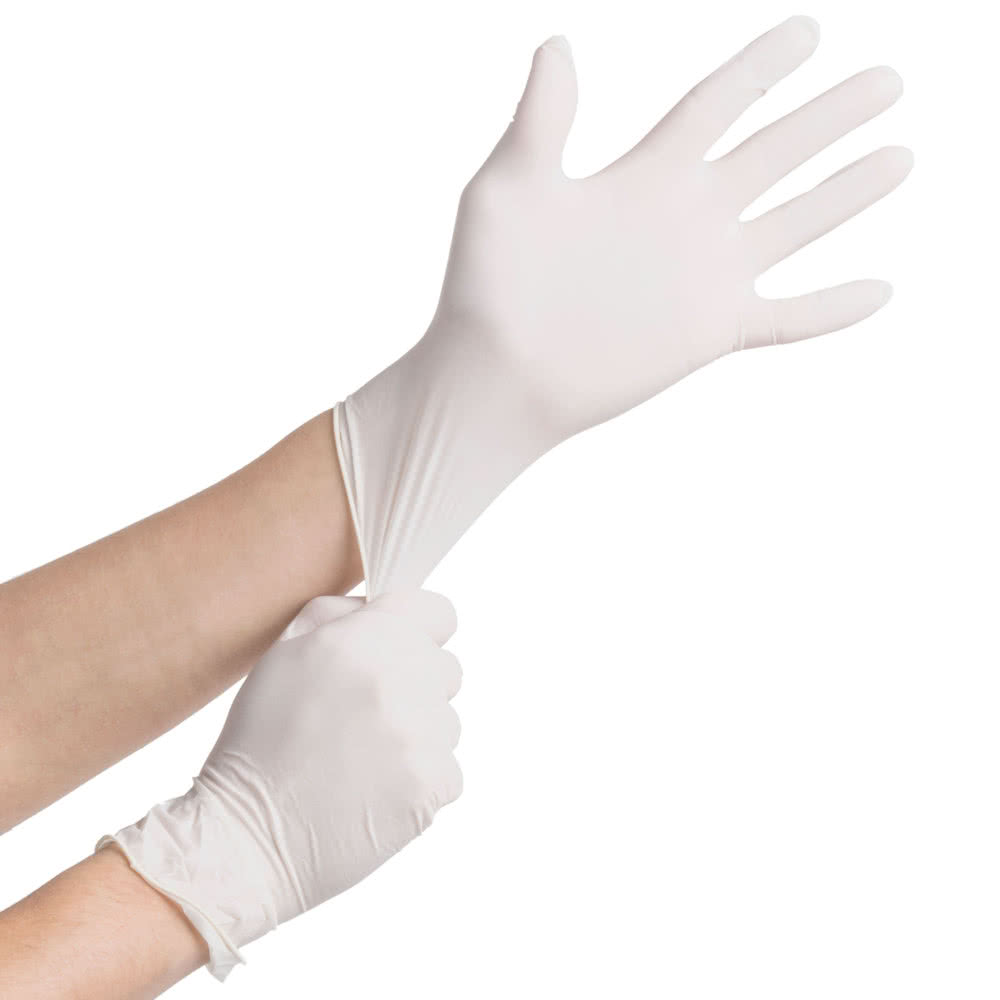
\includegraphics[scale= 0.3]{Images/Gloves.jpg}
    \caption{Vi gör oss redo för att använda Latex/Overleaf}
    \label{fig:latex}
\end{figure}


\begin{figure}[H]
    \centering
    
\includegraphics{Images/Approved.jpg}
    \caption{Damn, we got approved \citep{einstein}}
    \label{fig:chuckychuck}
\end{figure}


\begin{figure*}[t!]
    \centering
    \begin{subfigure}[t]{0.5\textwidth}
        \centering
        
\includegraphics[height=2.0in]{Images/Approved.jpg}
        \caption{Lorem ipsum}
    \end{subfigure}%
    ~ 
    \begin{subfigure}[t]{0.5\textwidth}
        \centering
        
\includegraphics[height=1.5in]{Images/Approved.jpg}
        \caption{Lorem ipsum, lorem ipsum,Lorem ipsum, lorem ipsum,Lorem ipsum}
    \end{subfigure}
    \caption{Caption place holder}
\end{figure*}


\begin{wrapfigure}{r}{0.5\textwidth}
  \begin{center}
    
\includegraphics[width=0.48\textwidth]{Images/Approved.jpg}
  \end{center}
  %\caption{HEJSAN HOPPSAN}
\end{wrapfigure}
\subsection{First Subsection in ``Second Section''}

\subsection{Second Subsection in ``Second Section''}

\subsubsection{First Subssubsection}

\subsubsection{Second Subsubsection}

\paragraph{First Paragraph}

\paragraph{Second Paragraph}


\section*{Section without numbering}

\subsection*{Subsection without numbering}

\subsubsection*{Subsubsection without numbering}
\begin{table}[H]
    \centering  
    \begin{tabular}{||c|r|l||}
        \hline 
        \textbf{Measurement using} & \textbf{Value} & \textbf{Error}\\ 
        \hline 
        SNZ  & 230 V & $\pm10^{-9000}$ V \\
        \hline
        Fluke & 215.6 V & $\pm20$ V \\
        \hline 
        Agilent & 232.1 V  & $\pm1.2$ V \\
        \hline 
        HPn & 231.3 V& $\pm0.01$ V \\
        \hline
        Z2 & 0 V & $>9000$ V \\
        \hline
        \end{tabular}
    \caption{Table from a report from Forkman}
    \label{Forkman_Mätning}
\end{table}


You don't gave to make tables such as this one from Forkman (\ref{Forkman_Mätning}), you can also make lists

\begin{enumerate}
    \item Dot 1
    \begin{enumerate}
        \item Dot 1a
        \item Dot 1b
    \end{enumerate}
\end{enumerate}

Or like this

\begin{itemize}
    \item Thing 1
    \item Thing 2
    \begin{itemize}
        \item Pinecone
        \item Pineapple
        \begin{itemize}
            \item I like Pines and SNZ
        \end{itemize}
    \end{itemize}
    \item Thing 3
    \item Thing 4
\end{itemize}

Or...

\begin{description}
    \item[Thing 1] Something 1a
    \item[Thing 2] Something 2a
\end{description}

Or like this

\begin{table}[H]
    \centering
    \begin{tabular}{r|c|l}
        Hi & ! & :D \\
        \hline
        THIS & IS & Tabular, not sparta \\
    \end{tabular}
    \caption{Box of things}
    \label{Mina_lådor_av_streck}
\end{table}


There exist a large library to make mathematical expressions in \LaTeX{}, where we will only go through a portion of them for you to familiarise your self with how it works.

\subsection{Symbols}

Many different symbols are available to use in \LaTeX{}, for example some common are:

\begin{equation}
    \textit{Just some mathimatical symbols}
\end{equation}
\begin{equation}
    \alpha, \beta, \gamma, \Gamma, \delta, \Delta, \varepsilon, \epsilon, \zeta, \eta, \Theta, \theta, \vartheta, \iota, \kappa, \varkappa, \Lambda, \lambda, \mu, \nu, \Xi
\end{equation}
\begin{equation}
    \xi, \Pi, \pi, \varpi, \rho, \varrho, \Sigma, \sigma, \varsigma, \tau, \Upsilon, \upsilon, \Phi, \phi, \varphi, \chi, \Psi, \psi, \Omega, \omega
\end{equation}

\subsection{Equations}

There are three main ways to write equations in latex, the first one is by writing one or two \$\$ signs between the equations:

$1+1=2$

$$
1-1=0
$$

You can also use the equation command in the command begin:

\begin{equation}\label{5_typ}
    2+3=5
\end{equation}

\eqref{5_typ} 
and without the numbering to the right

\begin{equation*}
    5-3 = 2
\end{equation*}

The last way is to use the align command, there as the name says. One can align the equations by using \{\}\& at the desired place to align each equation. (Obs every equation need to have it) Also to end an equation to be able to write an new equation bellow, one need to write $\backslash \backslash$ after the equation.

\begin{align}
    {}& \textit{Just som text...}\\
    {}& a = b + c\\
    {}& z = y + x\\
    \textit{This one is not alignend}
\end{align}

You can use all different kinds of things the math environment, bellow you can find a couple of examples, but it is best to google want you want or look at the latex wiki \href{https://en.wikibooks.org/wiki/LaTeX/Advanced_Mathematics}{LINK}


$$
\int^{\int^\int}_{\int_\int} \lim_{a \to \sum^{a}_{a}} \alpha \beta \gamma dt
$$

\begin{equation}
    SNZ_{cool}
    = \left(
    \lim_{SNZ \to 2 Cool 4 School} \int_{\beta}^\infty \sum_{\alpha = \beta}^{\gamma} \frac{10}{2} \cdot \frac{\pi}{\sqrt{\pi^2}}
    \right)^{Swag-i-skogen}
\end{equation}

\subsection{Other Math formulas}

Multiplications - Dot product or crossproduct

\begin{equation}
    A \times B
\end{equation}
\begin{equation}
    A \cdot B
\end{equation}

Fractions

\begin{equation}
    \frac{1}{2}
    = 0.5
\end{equation}

Matrices

$$
A = 
\begin{bmatrix}
    1 & 2 & 3 \\
    4 & 5 & 6 \\
    7 & 8 & 9 \\
\end{bmatrix}
, \qquad
b = 
\begin{bmatrix}
    10 \\
    11 \\
    12 \\
\end{bmatrix}
$$

Transpose

\begin{equation}
    A^\top
\end{equation}

Dynamic sizes of parenthesis

\begin{equation}
    \left(
    \frac{
    \left(
    \frac{\left(\frac{\left( a \right)}{b} \right) }{\left(\frac{c}{d} \right) }
    \right)
    }{d}
    \right)
\end{equation} 

Boxed in equations

\begin{equation}
    \boxed{
    x^2+y^2
    \neq (x + y)^2
    }
\end{equation}

And there are fun math too

\begin{align*}
    &\forall SNZ_{members} \exists (Cool_{members}  \subseteq SNZ_{members}) \in \mathbb{Z} \\
    &\land \\
    &\forall \mathbb{Z} \exists (Cool_{\mathbb{Z}}  \equiv SNZ_{members})
\end{align*}
%\newpage
%\section{Last Chapter: Fancy stuff}
%You do not always have to write .tex files for each chapter, however, they provide an easier overview of each individual part of the document. So for smaller reports etc. you can just as well write directly in main.tex, depending on how you want to do yourself, warning however if you write a lot it will be harder to keep track of what is what in the document.\\[5mm]
%A more bookish way of writing is to have 2 columns of text, this can be specified as the default at the beginning of the document or you can switch to and from more columns in the following way: \\[5mm]
%Warning, however, gives a new page.\twocolumn
\textbf{Example text lipsum}\\
\lipsum[1-5]
\onecolumn
\newpage

%====================================================
%   Litteraturförteckning via bib fil
%   vilket underlättar inmatning av källor till dokumentet.
\bibliography{Bibtex_file.bib}
\end{document}
